\documentclass[10pt,conference,twocolumn]{IEEEtran}
%\IEEEoverridecommandlockouts
% The preceding line is only needed to identify funding in the first footnote. \
%If that is unneeded, please comment it out.      
\usepackage{lipsum}
\usepackage{blindtext}
\usepackage{cite}
\usepackage{amsmath,amssymb,amsfonts}
\usepackage{algorithmic}
\usepackage{graphicx}
\usepackage{textcomp}
\usepackage{xcolor}
\def\BibTeX{{\rm B\kern-.05em{\sc i\kern-.025em b}\kern-.08em
    T\kern-.1667em\lower.7ex\hbox{E}\kern-.125emX}}
\DeclareMathOperator*{\argmax}{arg\,max}

\ifCLASSOPTIONcompsoc
\usepackage[caption=false,font=normalsize,labelfon
t=sf,textfont=sf]{subfig}
\else
\usepackage[caption=false,font=footnotesize]{subfi
g}
\fi

\title{Sequential Auction Assignment \thanks{A special mention to the MathSys 2018/19 Cohort, whose conversations and help in testing via the bot arena have been invaluable}}
\author{Richard Fox
\IEEEauthorblockA{\\ Mathematics for Real-World Systems Centre for Doctoral Training\\Warwick Mathematics Institute\\University of Warwick\\richard.fox@warwick.ac.uk}
}
\date{}



\usepackage[utf8]{inputenc}
\usepackage{titling}

\begin{document}

\maketitle

\begin{abstract}
   Four games are considered, falling into two categories of auction, in which the aim is to create a bidding bot that succeeds in an unknown environment. First, analysis of simple strategies are performed, to create a viable policy. Passive reinforcement learning is then applied to these viable policies to optimise them. In extensive local testing this bot performed very well, and in collaborative testing still remained competitive. Its performance in a completely unknown environment is still yet to be seen. Future work could include analysis of critical regret matching, replicator dynamics or an alternative learning paradigm.
\end{abstract}

\section{Introduction}

There are four auctions considered that fall within two types of auction, with two variations on each type, which are first to five and value accumulation. These require a bidder to accumulate a set number of items (in our case 5) of the same type after which the game ends, or to accumulate the highest number of points (sum of values of items owned) over the whole sequence of auctions, each auction is referred to as a round and there are $R$ rounds in a sequence. 


Formally, these are extensive-form finite games with imperfect information defined as a tuple,
$$\langle N, A, H, Z, \vec{i}, \vec{A},\sigma,\mathbf{u} \rangle , $$
that contains:
\begin{itemize}
    \item $N = \{1,\dots , n \}$ the set of bidders
    \item $A$ a set containing the possible actions
    \item $R$ a set containing the choice nodes, with exactly one root $r_0$
    \item $Z$ a set of leaf nodes (terminal states)
    \item $\vec{i} :R \rightarrow N$ a turn function, in this case turns are defined as each round of an auction 
    \item $\vec{A} : R \rightarrow 2^A$ mapping the choice nodes to the power-set of actions thereby fixing all the allowed actions
    \item $\sigma : R \times A \rightarrow R \cup Z$ a successor function, i.e. where an action at a choice node leads, either another choice node or a terminal state that we require to be injective
    \item $\mathbf{u} = (u_1,\dots,u_n)\quad u_i : Z \rightarrow \mathbb{R}$, $u_i$ is a utility function and $\mathbf{u}$ is each bidders utility function
\end{itemize}

with an injective $\sigma$ and a defined root $r_0$, can be expressed as a tree with branches for each choice node, the current choice node is indistinguishable from all others at the same level, and previous rounds are common knowledge\footnote{common knowledge is defined as knowledge that every individual knows, knows that every other individual knows, knows that they know that they and every other knows that they know this knowledge, ad infinitum }, as is the item sold and price paid for it, and the next round only depends on the current round. All finite extensive-form games have at least one Nash equilibrium (NE), brute force will not work to find it in this case, instead the approach is to simulate very simple strategies, including considerations of degeneracy, and analytically find profitable deviations from this. 

Equivalent bids are awarded randomly to one of the bidders who placed at bid at that price, first to five sequences end at $ r_{200}$ irrespective of if there is a winner by that point, value accumulation runs for a full 200 rounds and this allows for multiple players to have equivalent point totals. The bidders have a fixed sum of money to exchange for items, known as their budget $B_i \subseteq R$, where $B_i^{r_0} = 1000, \: \forall \: i \in N$. There is an assumption that the reader has a familiarity of the rules of the auctions examined in this assignment, but the details of which are explained in the Appendix otherwise.

Also, these games can be modelled as a Markov Decision Process (MDP), and, for completeness, more specifically as a Markov Reward Process (MRP). Unfortunately, the MDP state space is incredibly large \footnote{calculated with an indicative value for $\mid N \mid = 10$, and assuming every bidder spends all their money linearly throughout the rounds, giving average $B_i = 500$ so taking $\mid R \times A \mid \approx 200^{500}$} of order, $$\sim O\big(\mid N\mid^{ \mid R \times A \mid}\big) \sim 1*10^{100000}$$
meaning that while theoretically possible to use tools like backward induction\cite{textbook} or value iteration\cite{textbook} , it is highly impracticable to compute even a small fraction of this state space effectively. Due to this, the approach taken is to use reinforcement learning on a viable policy, which effectively truncates the state space to exploration around this policy\cite{RL}. 

First, we must assess what is a 'viable' policy by evaluating simple pure strategies, to create a robust mixed strategy. Creating such a policy is not as straightforward as one may think due to integer bids in a finite range and item values being globally fixed, leading to bid degeneracy and therefore a dependence on $\mid N\mid$. 

\begin{figure*}[!t]
\centering
\subfloat[No Degeneracy]{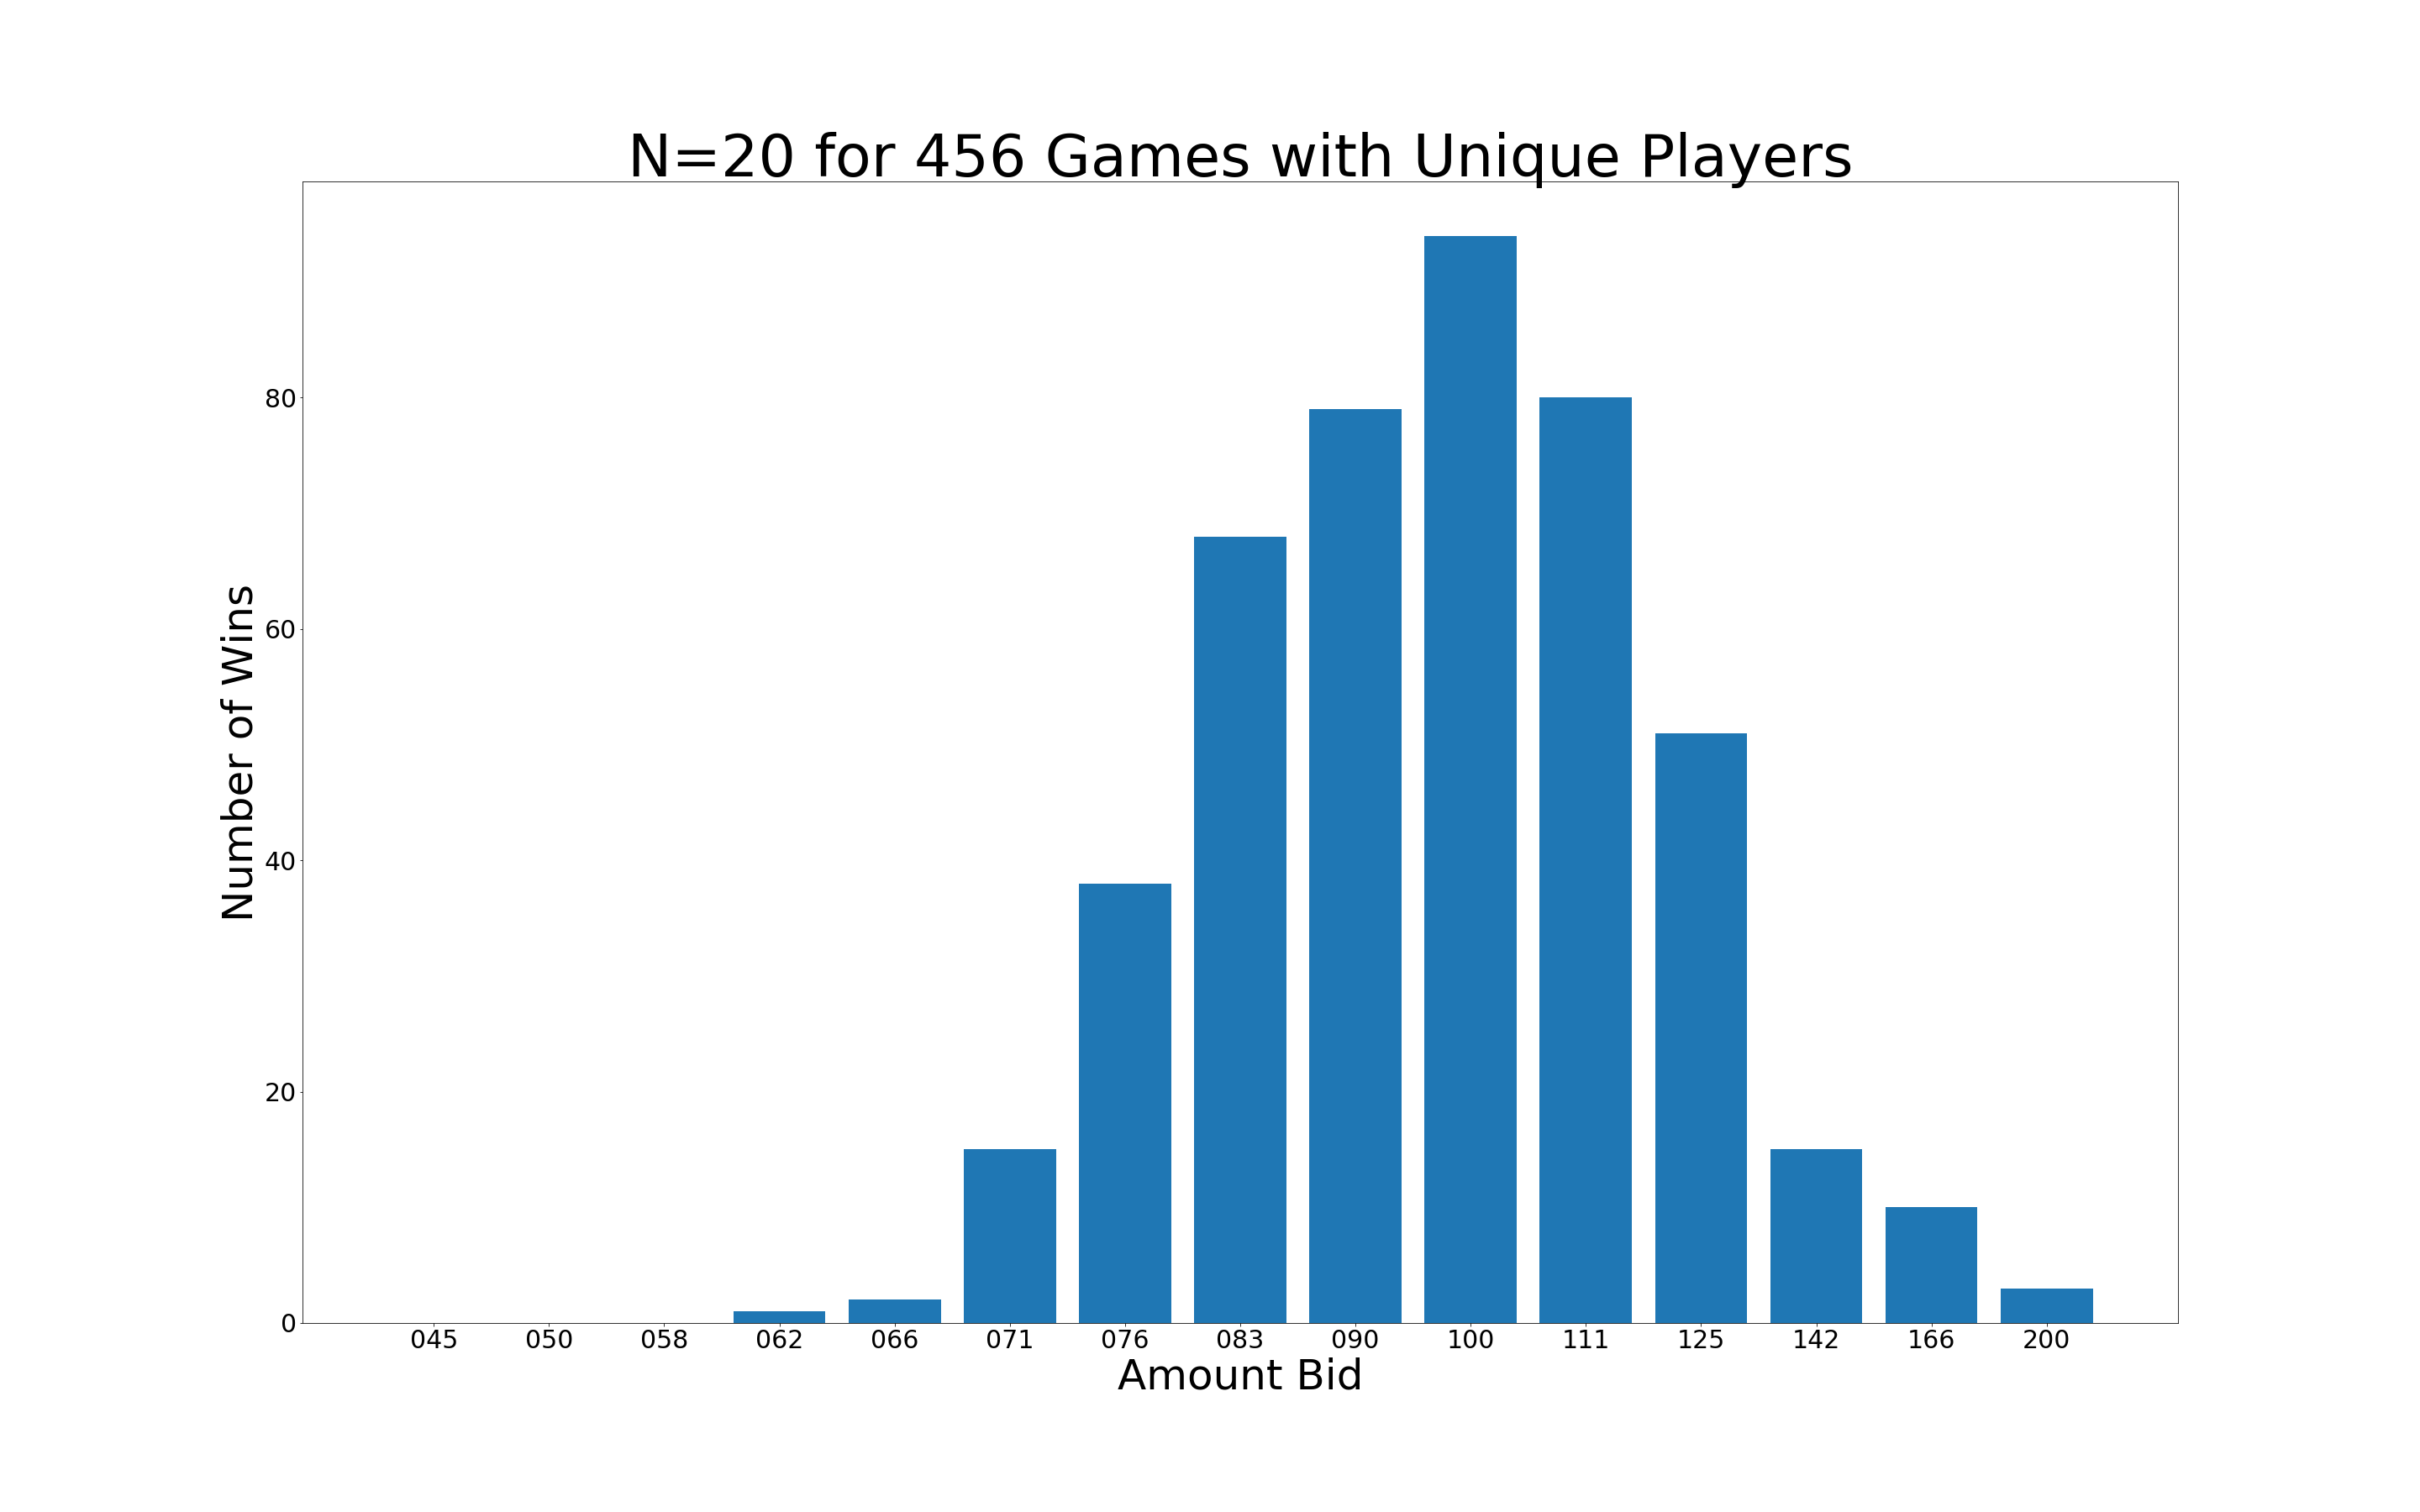
\includegraphics[width=.5\linewidth]{g1.png}}
\hfil
\subfloat[2x Degeneracy]{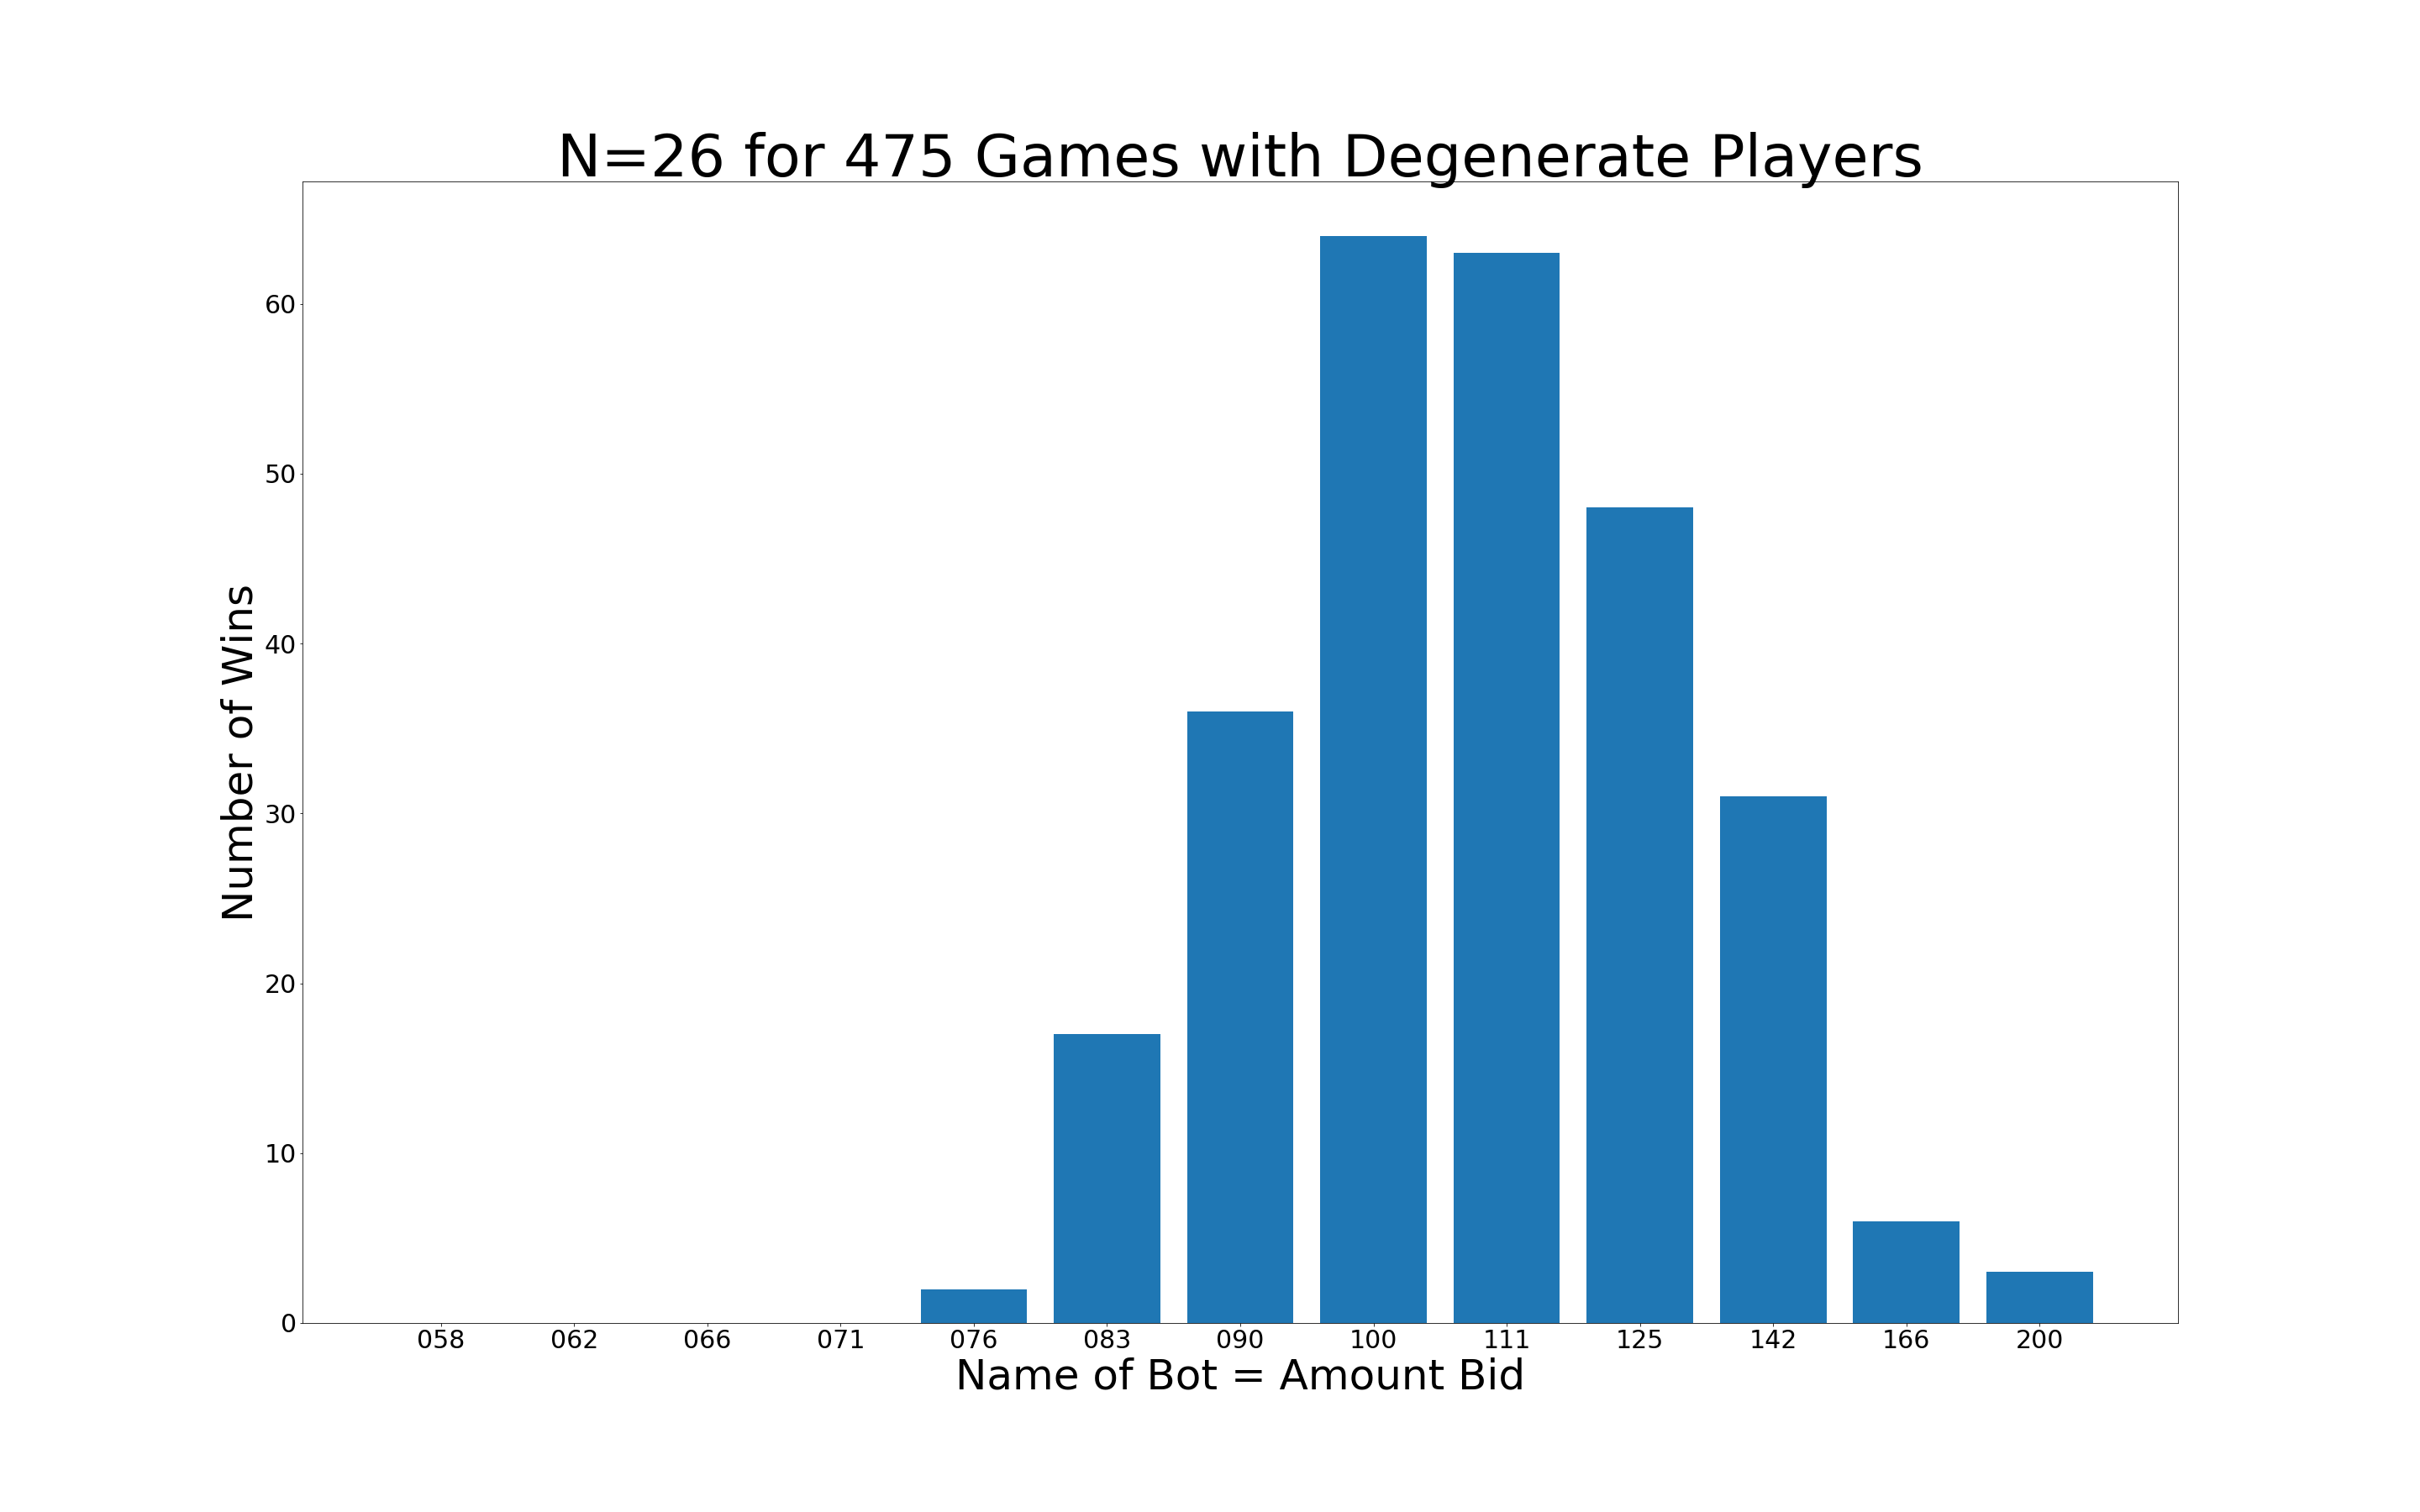
\includegraphics[width=.5\linewidth]{g2.png}}
\label{fig_sim}
\subfloat[3x Degeneracy]{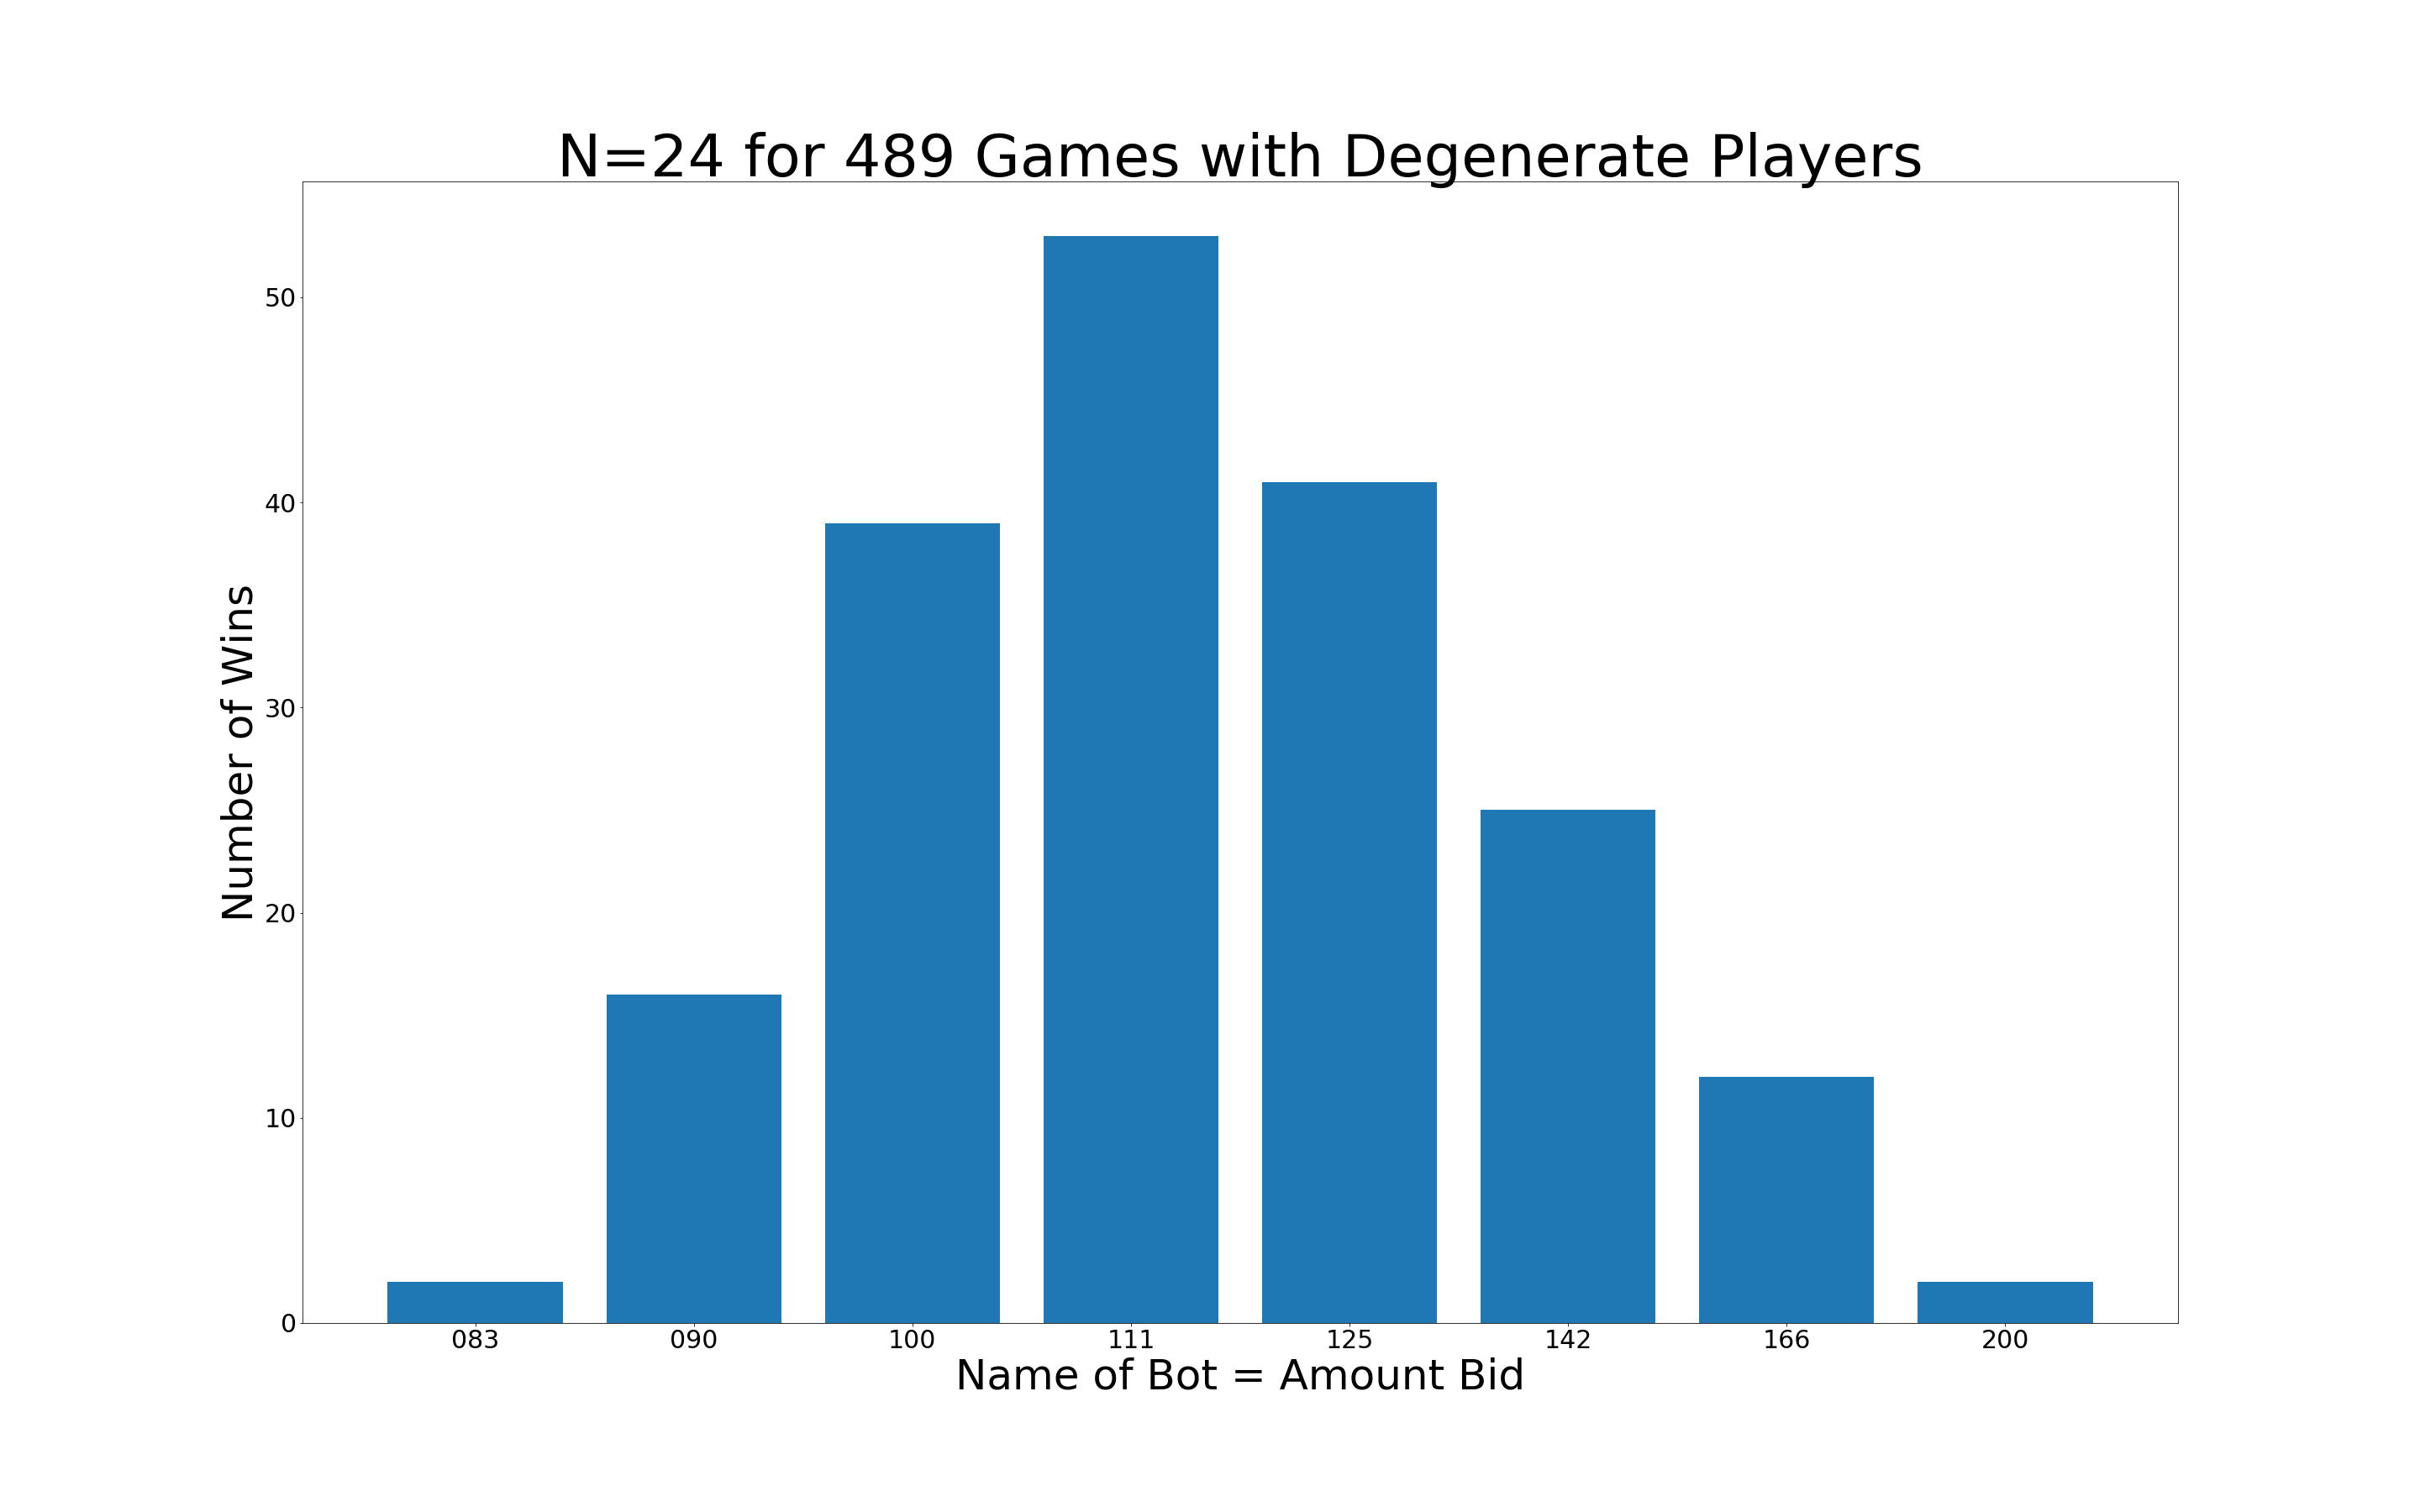
\includegraphics[width=.5\linewidth]{g3.png}}
\hfil
\subfloat[4x Degeneracy]{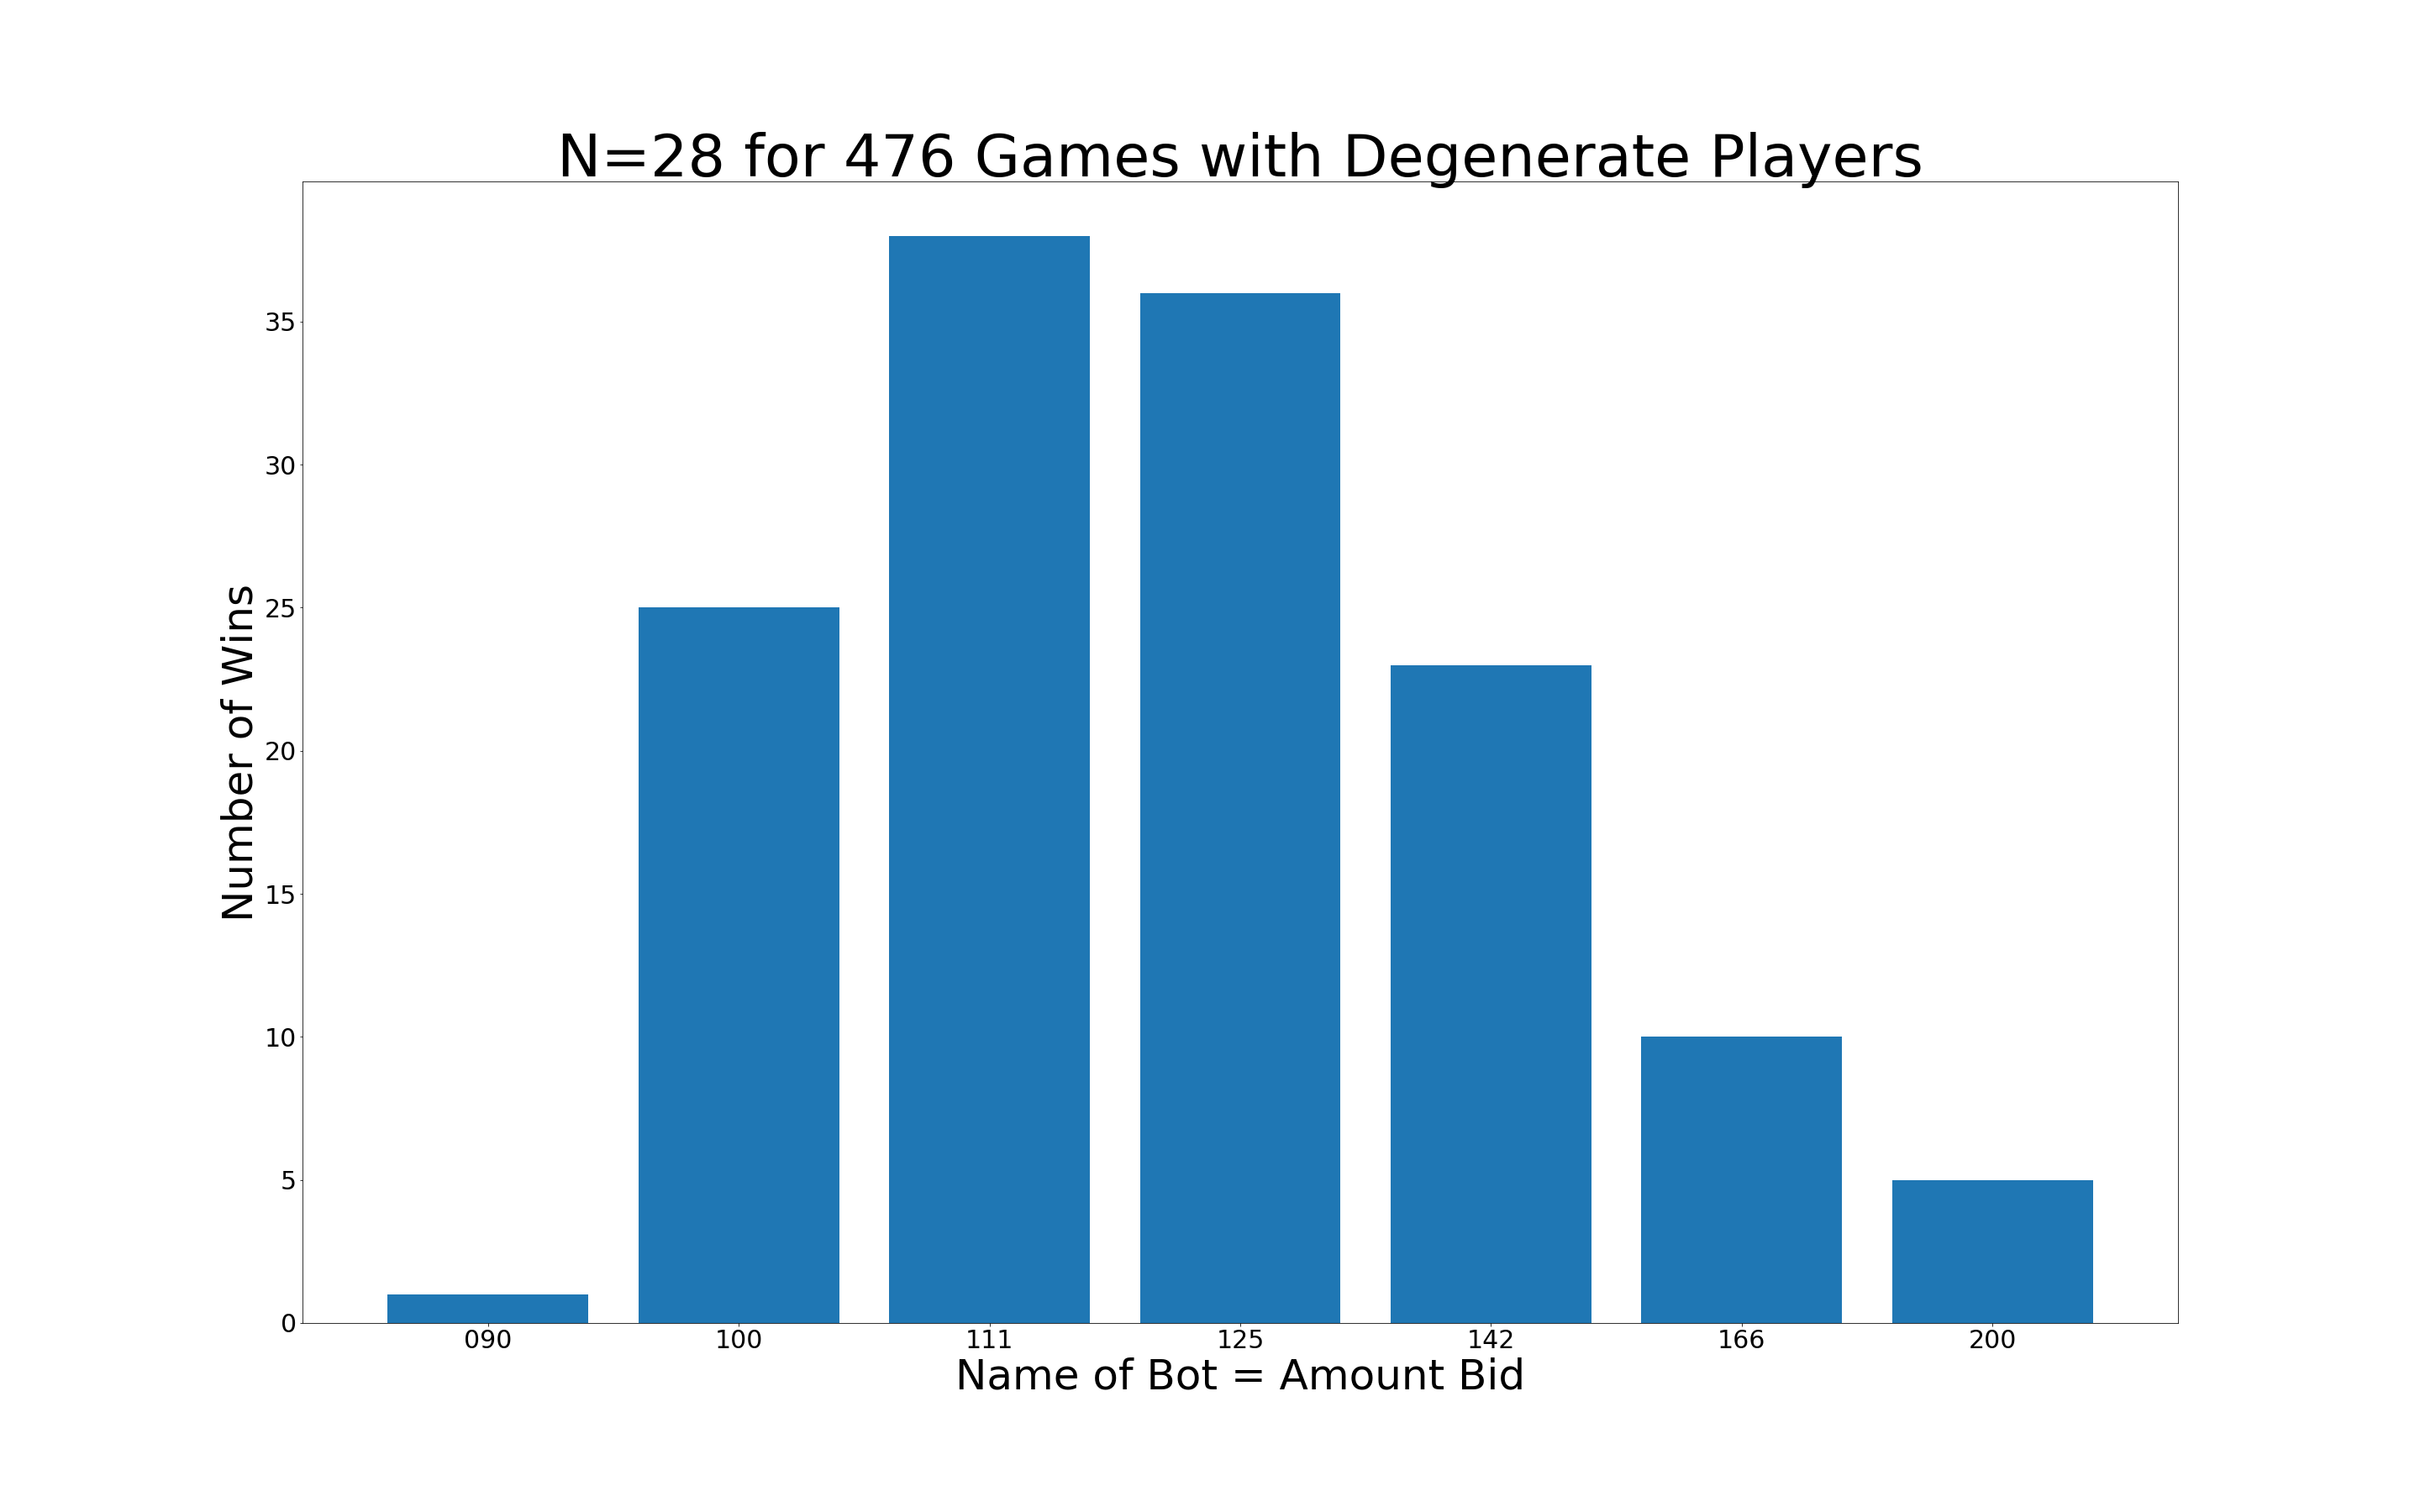
\includegraphics[width=.5\linewidth]{g4.png}}
\caption{Wins for each FlatBot$X$ over the course of $N=500$ games, the x axis labels refer to the $X$ value of the FlatBot. There are less than $N=500$ games completed due to rare games where no one wins or errors are thrown during the game}
\label{x}
\end{figure*}

Secondly, passive reinforcement learning is applied, after examining the differences between variations in order to exploit any particulars in each case. By using this technique it is hoped to gain insight into non-trivially analysed parameters, identified with the initial analytical approach. Whilst not as robust as it could be here, which is discussed later, there should either be significant improvements or a reasonable empirical proof of the viability of these strategies.


    
\section{First to Five}

\subsection{Analysis of Strategies}

Starting with bidders that bid the same amount each round is a simple strategy, known as 'FlatBot$X$' where $X$ is the amount bid, serving as a initial testing ground. Although, some considerations of the auction itself are applied, namely that if you need 5 items to win, then you must be able to bid on that many items meaning that no FlatBot above $X=200$ is considered. Conversely, as there are 4 types of item on offer there will be a maximum of 17 rounds before there are 5 of any type in a range, which relates to FlatBot$58$. Taking the maximum that can be bid consistently for $n_{expect}$ rounds $X = \frac{B_0}{n_{expect}}$, where $n_{expect}\in [5 \, .. \, 17]$, and ignoring bots that would not bid within 200 rounds, we populate our testing environment with the full range of these FlatBots, the increase in degeneracy shows a higher proficiency for higher $X$ Fig.\ref{x}.

 In this regime, the first profitable deviation considered is to only bid on the required type with FlatBot200. Although, with $g>4$  this is weak to smaller FlatBots as they can effectively 'spray and pray' for the type with the least amount of associated degeneracy. An increase in effectiveness can be achieved by looking for the next most frequent type, but this is now dependant on $g$, which is not known a priori and must be estimated, and when $g$ is over estimated, next highest frequency is weak to the first highest frequency strategy. Further to this there is another deviation that can be performed, that is to bid on the next most (or least or next least) frequent type depending on the degeneracy in the system, or to perform switching based on observed degeneracy, although this switch may also be degenerate. Switching implies one cannot use the FlatBot200 as this can only secure 5 items, and you should not pay less than 58, as this introduces unnecessary risk of being out bid. On the other hand switching can fall pray to a 'sting in the tail' FlatBot if not careful, that is a FlatBot that bids everything it has left if it already has 4 of this type.

As the level of degeneracy is environment dependant, a behavioural strategy is more applicable as want to adapt as more of a particular environment is deduced. Therefore what we want to learn is a distribution for the probability of which strategy is taken given the amount of amount of items bought for less than 200 and given the estimated amount of degenerate strategies. Therefore creating a much smaller state space to learn over.

\subsection{Variant Differences}
In the first variant of first to five, the list of items, in the correct order, is published to all participants. This allows for the possibility of interrogating this list to find the first five of any type to bid on. Unlike all other auctions examined here, the second variant restricts the information available, by removing the published order of items. 

The initial evaluation of FlatBots for the first to five auction does not take the item order into account, although the total number of each type of item is still available in both variants. Therefore, these two variant can be approached much the same, with the only difference being to evaluate frequency in a certain time period ahead, and to look for the most available item over all rounds. This approach is much weaker in the second variant as it cannot see unusually high entropy item order states, leading to a greater effectiveness of modified FlatBots.

This converges to almost the same states to learn over, with the first variant having the extra parameter of number of rounds in the future to evaluate. 

\section{Value Accumulation}
\subsection{Analysis of strategies}
Here, we start with calculating the total number of points available throughout the auction $v'$, by using the published list of items, and the published list of item values. Then, calculating the expected money per point value $v_{x_i} = \frac{B_{x_i}}{v'}$. Repeating this at the start of each round give a variable that scales with dwindling points available and when winning items and therefore accumulating points. Used with the items intrinsic value $v_{item}$, gives an individual their Value $V=v_{x_i}v_{item}$ for the item up for auction each round.

Now, this will obviously change contiguously for each bidder after each round Fig.\ref{ppp}, and decrease if is winning, however aggression now comes into play. In first to five auction, maximal aggression, even so far has to bitterly stop rivals bids, is displayed at all times, with value accumulation the approach needs endurance as it always, as long as everyone doesn't run out of money, completes the full 200 rounds. 

That said, aggression has its place here, as there is merit in paying a small amount more to secure points. The balance between aggression and endurance is very fine, and most if not all bidders will have varying levels of aggression, although there is plenty of information in the auction to try and fit to to extract this information, the approach is to wrap this up in stochastic noise.

\begin{figure}[!h]
    \centering
    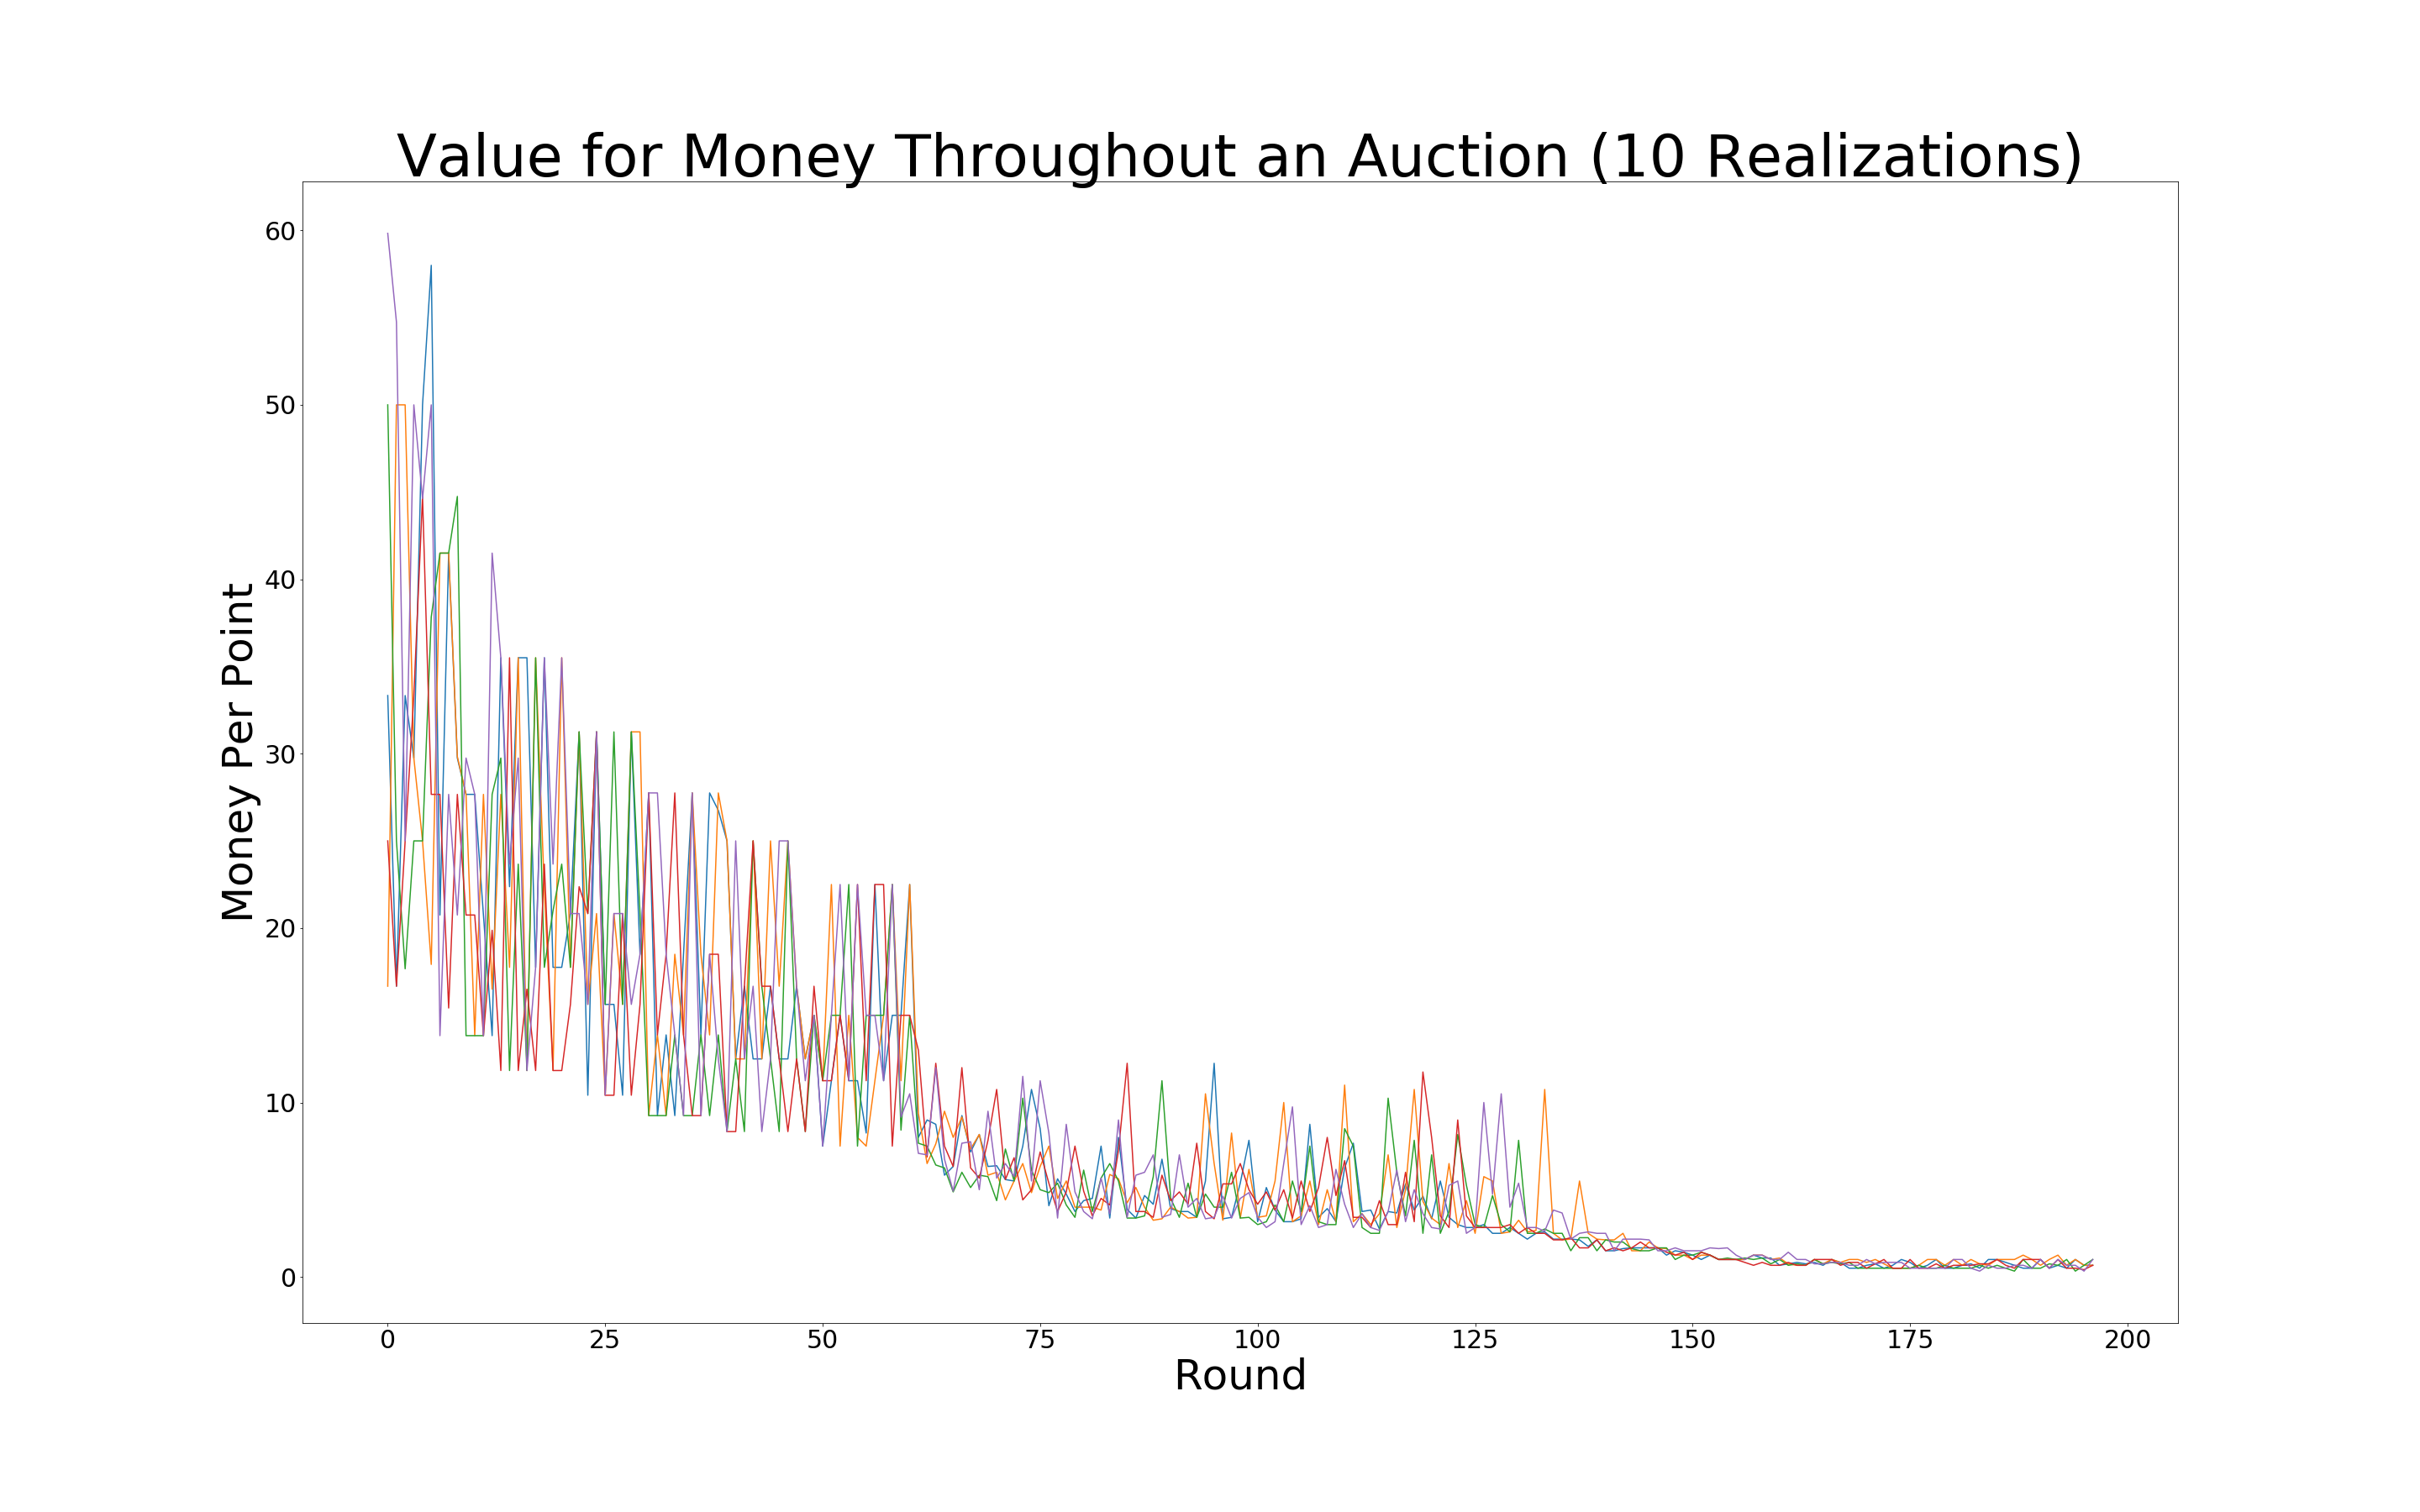
\includegraphics[width=\linewidth]{PPP.png}
    \caption{Typical spread of how many points are gained for each money spent throughout a sequence of rounds.}
    \label{ppp}
\end{figure}

Assume bids are approximated by a normal distribution around $V$ as the mean, that we will update throughout the rounds, we want to be bidding in the $[\sigma,2\sigma]$ range, where $\sigma =$ the standard deviation, region of the distributions probability density function. This means that a sufficient amount to be competitive in every round is bet, but not so much as to over pay and run out of money. As we are only in one realisation the statistic will be a sample, so each average taken will vary about the true average, with standard deviation $\sigma_{SEM}$. Thus, corrected by $\sigma = \sigma_{SEM} \sqrt{r_t}$ where $t=$ current round. As for own aggression this takes the simple form of a multiplicative constant that will be learned, here the level of aggression is proportional to consecutive wins/losses.

\subsection{Variant Differences}

The first variant is a sealed bid first price auction, as both variants of first to five are, which Vickrey showed in 1961\cite{Vickrey} to have a NE for an individual auction as $\frac{n-1}{n}V$. The second Variant is a second price auction, the winning bidder only pays what the second highest bidder bid, which is shown to have NE of $V$\cite{Vickrey}, i.e. to pay what the item is worth to you. All information provided in both auction variants is the exact same.

For both variants the NE from the literature is used as a baseline and apply the variance analysis and the aggression multiplier, with a view to having the RL also learn how to compensate for unreliable statistics before a sufficient number of rounds has pasted.

\section{Reinforcement Learning (RL)}
\subsection{Theory}
By the use of the passive adjective, it is implied that there is a preexisting policy (defined in previous sections) upon which temporal difference leaning is applied (3a), comparing to deviations from this policy with a deviation rate of $(1-\epsilon), \: \epsilon \in [0,1]$.

$$ V^{\pi}(s) = V^{\pi}(s) + \alpha[r(s) + \gamma V^{\pi}(s')-V^{\pi}(s)]$$

$$V^{\pi}(s) = \mathbb{E}_{Utility}\bigg[ \sum_{t=0}^R \gamma^t r(s_t) \bigg]$$

where $V^{\pi}(s)$ is the value of the policy in state $s$, $\alpha$ is a weighing constant that determines learning rate based on our confidence that the new policy is defacto an improvement, $\gamma$ a discounting term that controls the importance of future state values, $r(s)$ is the reward received in state $s$ and $\mathbb{E}_{Utility}$ is the expected utility \cite{RLtextbook}.

Values for terminal states is defined as well as rewards at each state, the value is then back-propagated in a Bellman Equation (value iteration) -esque manner. The optimal policy $\pi_s^*$ is defined as the policy that maximises value in each state as such:
$$\pi_s^* = \argmax_{\pi} V^{\pi}(s).$$

In addition to the selection of architecture for learning, there are different forms of input perception, defined as: Independent Learners, that look at their own actions and the associated rewards, Joint Action Learners, that also take into account all the other agents and Gradient based optimisation, that sits in the spectrum somewhere between the two. Here we take the Independent approach.

\subsection{Implementation}
A script to perform passive RL is created, also a file creating the policy that both the RL script reads from and updates and the actual played policy is drawn from. This take the form as a list of parameters that each have their own exploration rate $\epsilon$, but all have the same weighting $\alpha = 0.5$. No parameter is used in every game and are therefore updated when in the appropriate auction, hence the necessity of individual exploration rates.

In the first to five regime, it is imperative to win as soon as possible and therefore if we set the value of negligible importance $\epsilon_{import} = 0.01$, then we want: $$\gamma^{\mathbb{E}[r]} =\epsilon_{import}, \quad \gamma = \sqrt[\leftroot{-1}\uproot{2}\scriptstyle {\mathbb{E}[r]}]{\epsilon_{import}}$$ where $\mathbb{E}[r],\: r<R \: , \: r \in \mathbb{Z}^+$, is the expected number of rounds as discussed in section II.B, for example $\gamma \approx 0.76$ sets states $>17$ rounds in the future as negligible. In value accumulation a win is only dependant on the outcome of all rounds, therefore $\gamma = 1$. 

In the learning environment meant, there were a varying number of players of varying complexity, being randomly selected at the beginning of each round. In the submission of the work the value of parameters that is converged upon will be hard coded in, i.e. will not be dynamically leaning whilst playing, due to submission constraints.

\section{Conclusions \& Future Work}

During individual testing this converged policy has performed very well, less so in collaborative testing, but is for the most part competitive. The work submitted as part of this assignment uses the best policy achieved, there is not formal proof that this policy has not fallen prey to optimising in a local minima. Indeed it is highly likely not to be, as the state space is vast, there is a requirement for very extensive testing and input from a cross-disciplinary team of researchers to be declared solved in any sense. That said, I believe what has been achieved is in some sense "good" or in some approximation "competitive".

Going forward the obvious step is to take a gradient based approach to learning. In a slightly different direction, taking other analytical polices and trying to optimise them, in a similar approach to performed here and comparing to this one. Further to this, evaluate replicator dynamics to find the evolutionary stable strategies (ESS) that are emergent from policies that are competitive, but may only have a small probabilistic advantage. Studies of such dynamical systems lead to the establishing of critical points of convergence, which may be a more appropriate way to truncate the state space.

A more game theoretic alternative would be to apply critical regret matching (CRM), where there is further punishment for not taking actions that would have won a round and are available to that bidder in a certain state. Learning the opponents strategy this way could lead to a much more adaptive strategy, for instance that can consider $\mid N \mid$ dependence, which is mentioned above but never taken into serious consideration.

\begin{thebibliography}{9}

\bibitem{textbook}
Y. Shoham and K. Leyton-Brown, Multiagent systems. Cambridge: Cambridge Univ. Press, 2012.

\bibitem{RL}
Pineau and N. Roy, "Reinforcement learning with limited reinforcement: Using Bayes risk for active learning in POMDPs", Artificial Intelligence, vol. 187-188, pp. 115-132, 2012. Available: 10.1016/j.artint.2012.04.006.

\bibitem{Vickrey}
W. Vickrey, "Counterspeculation, Auctions, and Competitive Sealed Tenders", The Journal of Finance, vol. 16, no. 1, p. 8, 1961. Available: 10.2307/2977633.

\bibitem{RLtextbook}
S. Russell and P. Norvig, Artificial intelligence.

\end{thebibliography}

\appendix[Assignment and Game details (on next page)]

\begin{figure*}[!h]
\centering
\subfloat{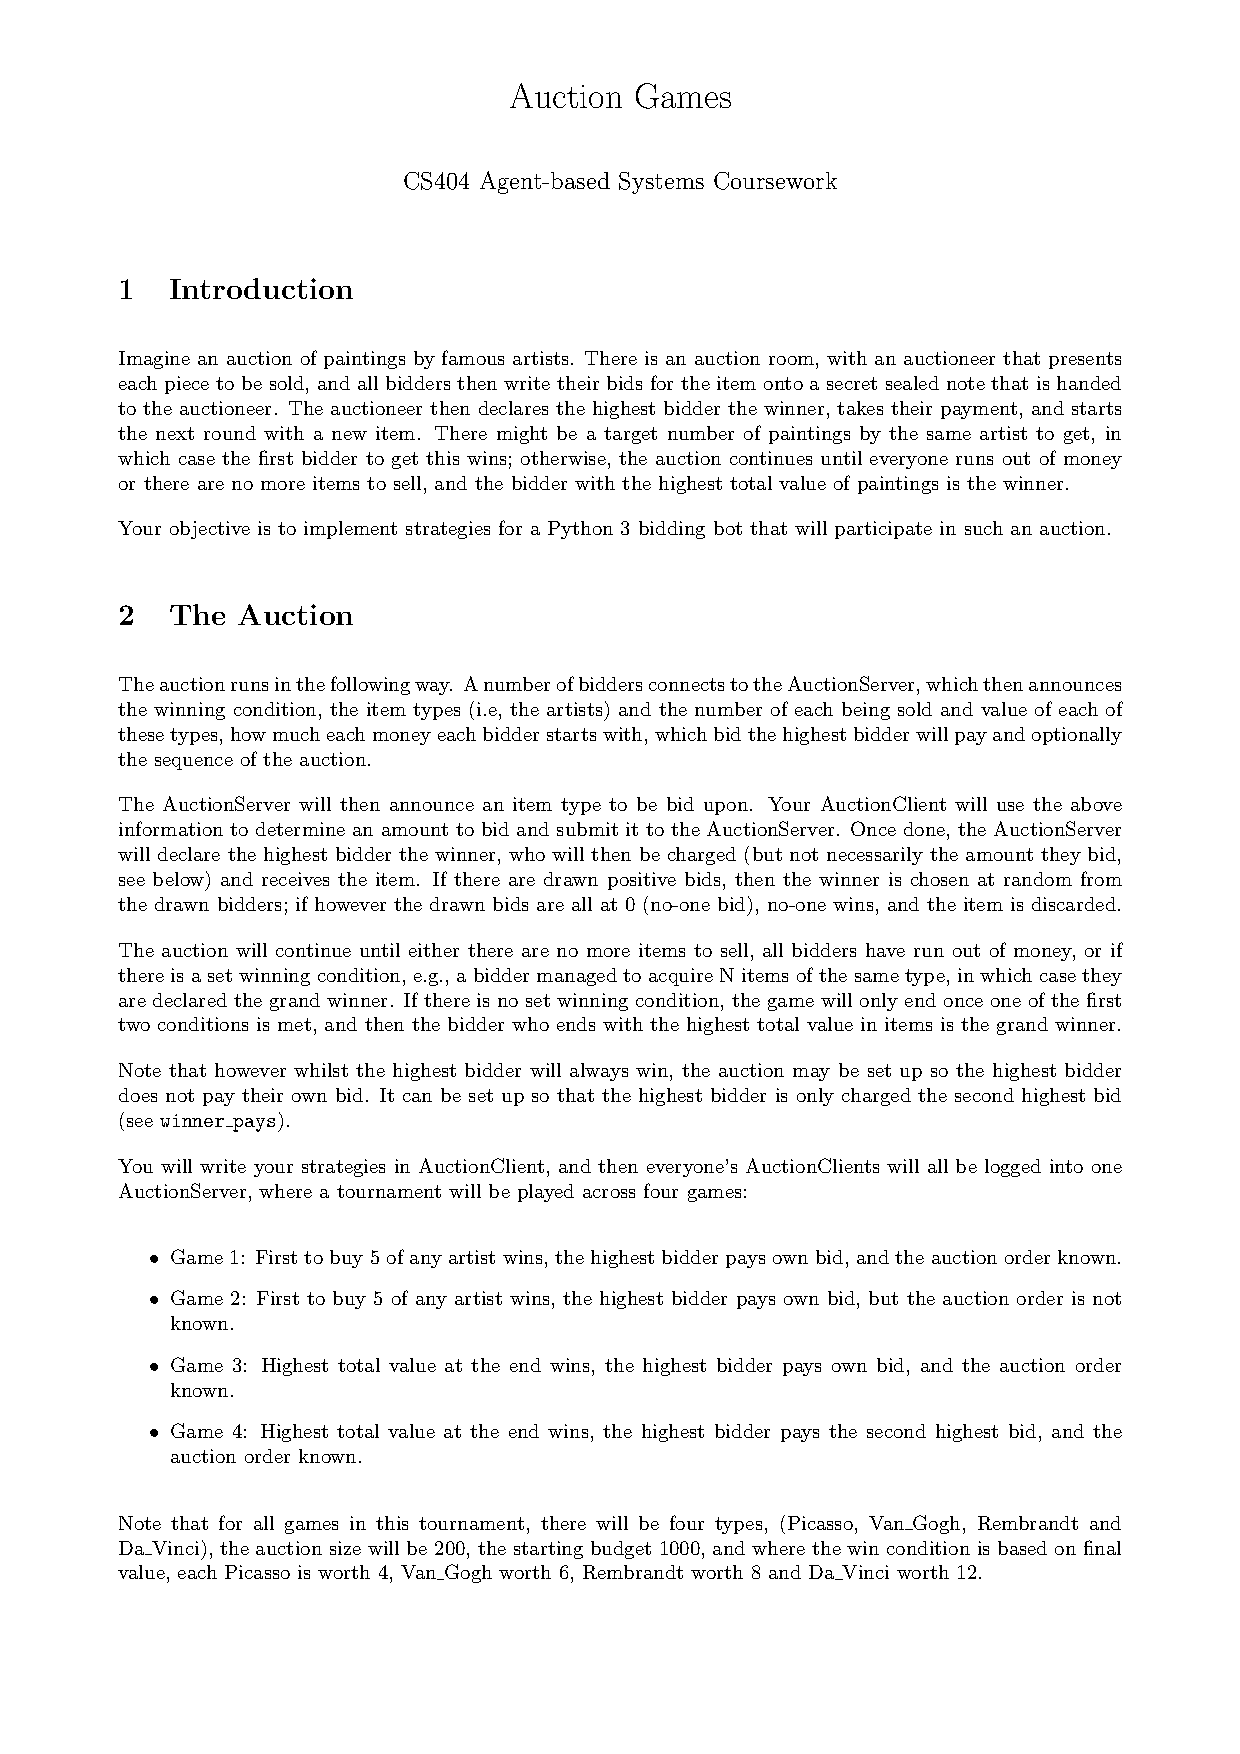
\includegraphics[page=1,width=0.5\textwidth]{spec19.pdf}}
\hfil
\subfloat{\includegraphics[page=2,width=0.5\textwidth]{spec19.pdf}}
\subfloat{\includegraphics[page=3,width=0.5\textwidth]{spec19.pdf}}
\end{figure*}



\end{document}
